% \documentclass[12pt, twoside]{article}
\usepackage[letterpaper, margin=1in, headsep=0.2in]{geometry}
\setlength{\headheight}{0.6in}
%\usepackage[english]{babel}
\usepackage[utf8]{inputenc}
\usepackage{microtype}
\usepackage{amsmath}
\usepackage{amssymb}
%\usepackage{amsfonts}
\usepackage[nomessages]{fp} %\FPeval{\var-name}{2*sin(pi/6)}
\usepackage{siunitx} %units in math. eg 20\milli\meter
\usepackage{yhmath} % for arcs, overparenth command
\usepackage{tikz} %graphics
\usetikzlibrary{quotes, angles, arrows, arrows.meta}
\usepackage{graphicx} %consider setting \graphicspath{{images/}}
\usepackage{parskip} %no paragraph indent
\usepackage{enumitem}
\usepackage{multicol}
\usepackage{venndiagram}

\usepackage{fancyhdr}
\pagestyle{fancy}
\fancyhf{}
\renewcommand{\headrulewidth}{0pt} % disable the underline of the header
\raggedbottom
\hfuzz=2mm %suppresses overfull box warnings

\usepackage{hyperref}

\fancyhead[LE]{\thepage}
\fancyhead[RO]{\thepage \\ Name: \hspace{4cm} \,\\}
\fancyhead[LO]{BECA / Dr. Huson / Geometry\\*  Unit 1: Segments, length, and area\\* 19 Sept 2022}

\begin{document}

\subsubsection*{1.9 Rounding and circle area}
\begin{enumerate}
\item Write in your notebook the formulas for the area and circumference of circles and these definitions:
\begin{itemize}
  \item The radius, $r$, is the distance from the center to the edge of a circle. 
  \item The diameter, $D$, is the distance all of the way across a circle, two times the radius. $D=2r$. 
  \item The circumference, $C$, is the distance around the circle (its perimeter).
  
\end{itemize}
  \[A=\pi r^2\]
  \[C=\pi D = 2\pi r\]
  
\item Given the circle centered at $O$ with radius $r=3$. Leave an exact answer, in terms of $\pi$ if necessary.
  \begin{multicols}{2}
    \begin{enumerate}
      \item Find the circumference of circle $O$. %\vspace{1cm}
      \item Find the area of the circle.\vspace{2cm}
    \end{enumerate}
    %\columnbreak
    \begin{tikzpicture}[scale=.635]
      \draw [help lines] (-5,-4) grid (5,4);
      %\draw [thick, ->] (-2.2,0) -- (10.4,0) node [below right] {$x$};
      %\draw [thick, ->] (0,-2.2)--(0,10.4) node [left] {$y$};
      \draw (0,0) circle [radius=3] node[below]{$O$};
      \draw [fill] (0,0) circle [radius=0.05];
    \end{tikzpicture}
  \end{multicols}

\item Find the area $A$ and circumference $C$ of a circle with radius 4 meters (in terms of $\pi$). 

\item Find the area $A$ and circumference $C$ of a circle with radius 5 feet (in terms of $\pi$). 
  
\newpage
    
\item Find the area of the shape shown below composed of a rectangle and circular cap. Leave your answer as an exact value in terms of $\pi$.
\begin{flushright}
\begin{tikzpicture}[scale=.635]
  \draw [help lines] (-2,-1) grid (8,7);
  \draw [thick, ->] (-2.2,0) -- (8.4,0) node [below right] {$x$};
  \draw [thick, ->] (0,-1.2)--(0,7.4) node [left] {$y$};
  \draw [thick] (1,1)--(7,1)--(7,3)--(1,3)--cycle;
  %\draw [thick] (3,4) arc (90:270:1);
  \draw [thick] (7,3) arc (0:180:3);
\end{tikzpicture}
\end{flushright}

\item Given the circle centered at $A$ with radius $r=2$. Leave an exact answer, in terms of $\pi$ if necessary.
  \begin{multicols}{2}
    \begin{enumerate}
      \item Find the circumference of circle $A$. %\vspace{1cm}
      \item Find the area of the circle.\vspace{2cm}
    \end{enumerate}
    %\columnbreak
    \begin{flushright}
    \begin{tikzpicture}[scale=.635]
      \draw [help lines] (-4,-4) grid (4,4);
      %\draw [thick, ->] (-2.2,0) -- (10.4,0) node [below right] {$x$};
      %\draw [thick, ->] (0,-2.2)--(0,10.4) node [left] {$y$};
      \draw (0,0) circle [radius=2] node[below]{$A$};
      \draw [fill] (0,0) circle [radius=0.05];
    \end{tikzpicture}
  \end{flushright}
  \end{multicols}

\item Find the area of the shape shown below composed of a rectangle and circular cap. Leave your answer as an exact value in terms of $\pi$.
\begin{flushright}
\begin{tikzpicture}[scale=.635]
  \draw [help lines] (-1,-1) grid (7,7);
  \draw [thick, ->] (-1.2,0) -- (7.4,0) node [below right] {$x$};
  \draw [thick, ->] (0,-1.2)--(0,7.4) node [left] {$y$};
  \draw [thick] (1,1)--(5,1)--(5,4)--(1,4)--cycle;
  %\draw [thick] (3,4) arc (90:270:1);
  \draw [thick] (5,4) arc (0:180:2);
\end{tikzpicture}
\end{flushright}


\end{enumerate}
\end{document}